%%%%%%%%%%%%%%%%%%%%%%%%%%%%%%%%%%%%%%%%%%%%%%
% Head matter - can we try to be consistent on
% included packages
\documentclass{beamer}
\mode<presentation>
{\usetheme{default}
 \usecolortheme{default}
 \usefonttheme{default}
 \setbeamertemplate{navigation symbols}{}
 \setbeamertemplate{footline}[frame number]
% \setbeamertemplate{caption}[numbered]
 }
\usepackage[english]{babel}
\usepackage{algorithm}
\usepackage[noend]{algpseudocode}
\usepackage[utf8x]{inputenc}
\usepackage{graphicx}
\usepackage{hyperref}
%\graphicspath{{./images/}}
\usepackage{tikz}
\usetikzlibrary{shapes.geometric, arrows,chains}
\usepackage{booktabs,makecell,multirow,tabularx}
\usepackage{verbatim}
\renewcommand{\arraystretch}{1.2}
\renewcommand\theadfont{\normalfont\bfseries}
\usepackage{array}
\usepackage{listings}
\lstset{language=Java, showstringspaces=false}
\usepackage[normalem]{ulem}
\usepackage{bm}
\def\layersep{2.5cm}

\usepackage{xcolor}
%\usepackage{subfig}
\setbeamertemplate{caption}{\insertcaption}
\usepackage[caption=false]{subfig}
\usepackage{hyperref}
\usepackage{verbatim}
%\setbeamertemplate{caption}[numbered]%\numberwithin{figure}{section}
% Define block styles

\usetheme{Copenhagen}
\hypersetup{pdfstartview={Fit}}
\lstset{basicstyle=\small\ttfamily,breaklines=true}

\usepackage{xmpmulti}

\tikzstyle{decision} = [diamond, draw, fill=blue!20, 
    text width=4.5em, text badly centered, node distance=3cm, inner sep=0pt]
\tikzstyle{block} = [rectangle, draw, fill=blue!20, 
    text width=3em, text centered, rounded corners, minimum height=3em]
\tikzstyle{line} = [draw, -latex']
\tikzstyle{cloud} = [draw, ellipse, fill=red!20, node distance=3cm,
    minimum height=2em]
\tikzset{
  startstop/.style={
    rectangle, 
    rounded corners,
    minimum width=3cm, 
    minimum height=1cm,
    align=center, 
    draw=black, 
    fill=red!30
    },
  process/.style={
    rectangle, 
    minimum width=3cm, 
    minimum height=1cm, 
    align=center, 
    draw=black, 
    fill=blue!30
    },
  decision/.style={
    rectangle, 
    minimum width=3cm, 
    minimum height=1cm, align=center, 
    draw=black, 
    fill=green!30
    },
  arrow/.style={thick,->,>=stealth},
  dec/.style={
    ellipse, 
    align=center, 
    draw=black, 
    fill=green!30
    },
}
\tikzstyle{arrow} = [thick,->,>=stealth]

\tikzset{onslide/.code args={<#1>#2}{%
  \only<#1>{\pgfkeysalso{#2}} % \pgfkeysalso doesn't change the path
}}

\makeatletter
\newenvironment<>{btHighlight}[1][]
{\begin{onlyenv}#2\begingroup\tikzset{bt@Highlight@par/.style={#1}}\begin{lrbox}{\@tempboxa}}
{\end{lrbox}\bt@HL@box[bt@Highlight@par]{\@tempboxa}\endgroup\end{onlyenv}}

\newcommand<>\btHL[1][]{%
  \only#2{\begin{btHighlight}[#1]\bgroup\aftergroup\bt@HL@endenv}%
}
\def\bt@HL@endenv{%
  \end{btHighlight}%   
  \egroup
}
\newcommand{\bt@HL@box}[2][]{%
  \tikz[#1]{%
    \pgfpathrectangle{\pgfpoint{1pt}{0pt}}{\pgfpoint{\wd #2}{\ht #2}}%
    \pgfusepath{use as bounding box}%
    \node[anchor=base west, fill=orange!30,outer sep=0pt,inner xsep=1pt, inner ysep=0pt, rounded corners=3pt, minimum height=\ht\strutbox+1pt,#1]{\raisebox{1pt}{\strut}\strut\usebox{#2}};
  }%
}
\makeatother

\definecolor{darkblue}{RGB}{37,55,97}
\definecolor{mellowyellow}{RGB}{247,206,70}
\definecolor{almostwhite}{RGB}{254,255,255}
\definecolor{merrygreen}{RGB}{79,173,91}
\definecolor{funkyorange}{RGB}{240,154,56}

\addtobeamertemplate{footnote}{\hskip -2em}{}
\newcommand\blfootnote[1]{%
  \begingroup
  \renewcommand\thefootnote{}\footnote{#1}%
  \addtocounter{footnote}{-1}%
  \endgroup
}

\DeclareMathOperator{\softmax}{softmax}
\DeclareMathOperator{\ReLU}{ReLU}

%%%%%%%%%%%%%%%%%%%%%%%%%%%%%%%%%%%%%%%%%%%%%%
% Formatting for title page
\title[LSTMs and GRUs]{Long Short Term Memories and Gated Recurrent Units}
\author{Jonathon Hare}
\institute[]
{
  Vision, Learning and Control\\
  University of Southampton 
}
\date{}
\subject{Computer Science}
\useoutertheme{infolines}
\setbeamertemplate{headline}{} %remove headline
\setbeamertemplate{navigation symbols}{} %remove navigation symbols
%%%%%%%%%%%%%%%%%%%%%%%%%%%%%%%%%%%%%%%%%%%%%%

\begin{document}

\begin{frame}[plain]
        \begin{tikzpicture}[overlay, remember picture, shift={(current page.south west)},font={\fontfamily{Montserrat-TOsF}\selectfont}]
        \fill [merrygreen,text=almostwhite] (0,0) rectangle (\paperwidth, \paperheight);
        \draw (5.5,7) node [align=left,text=almostwhite] {\Huge 
        \begin{tabular}{l} 
        \textbf{Forget} \textbf{to} \textbf{remember} \\
        \textbf{Remember} \textbf{to} \textbf{forget} 
        \end{tabular}};
        \draw (11,1) node [align=left,text=almostwhite] {\includegraphics[scale=0.15]{../vlc.png}};
        \end{tikzpicture}
\end{frame}

\begin{frame}
  \titlepage
  \tiny{Many of the images and animations used here were made by Adam Pr\"ugel-Bennett.}
\end{frame}
%-------------------------------------------------------------%

\begin{frame}
\frametitle{Recap: An RNN is just a recursive function invocation}

\begin{itemize}
  \item<1-> $\bm{y}(t) = \bm{f}(\bm{x}(t), \bm{c}(t-1)|\bm{W})$
  \item<1-> and the state $\bm{c}(t) = \bm{g}(\bm{x}(t), \bm{c}(t-1)|\bm{W})$
  \item<1-> If the output $\bm{y}(t)$ depends on the input
    $\bm{x}(t-2)$, then prediction will be
    \begin{align*}
      \bm{f}(\bm{x}(t), \bm{g}(\bm{x}(t), \bm{g}(\bm{x}(t-1), \bm{g}(\bm{x}(t-2)|\bm{W}), \bm{W}), \bm{W}), \bm{W})
    \end{align*}
  \item<1-> it should be clear that the gradients of this with respect to the weights can be found with the chain rule
  \item<2-> The back-propagated error will involve applying $\bm{f}$ multiple times
  \item<3-> Each time the error will get multiplied by some factor $a$
  \item<4-> If $\bm{y}(t)$ depends on the input $\bm{x}(t-\tau)$ then the back-propagated signal will be proportional to $a^{\tau-1}$
  \item<5-> This either vanishes or explodes when $\tau$ becomes large
\end{itemize}
\end{frame}

%-------------------------------------------------------------%

\begin{frame}
\frametitle{Vanishing and Exploding Gradients}
\begin{center}
  \multiinclude[<+>][format=pdf, graphics={width=\linewidth}] {recurrentVanish}
\end{center}
\end{frame}

%-------------------------------------------------------------%

\begin{frame}
  \frametitle{LSTM Architecture}

  \begin{itemize}
  \item<+-> LSTMs (long-short term memory) was designed to solve this problem
  \item<+-> Key ideas: to retain a `long-term memory' requires
    \begin{align*}
      \bm{c}(t) = \bm{c}(t-1)
    \end{align*}
  \item<+-> Sometimes we have to forget and sometimes we have to change a memory
  \item<+-> To do this we should use `gates' that saturate at 0 and 1
  \item<+-> Sigmoid functions naturally saturate at 0 and 1
  \end{itemize}

\end{frame}

%-------------------------------------------------------------%

\begin{frame}
\frametitle{LSTM Architecture}
\begin{center}
  \multiinclude[<+>][format=pdf, graphics={width=0.85\linewidth}] {lstm-dyn}
\end{center}
\end{frame}

%-------------------------------------------------------------%

\begin{frame}
\frametitle{Update Equations}

  \begin{itemize}
  \item<+-> Inputs $\bm{z}(t) = \left(\strut \bm{x}(t),\, \bm{h}(t-1)\right)$
  \item<+-> Network updates ($\bm{W}_*$ are the free parameters)
    \begin{align*}
      \bm{f}(t) &= \bm{\sigma}\!\left( \bm{W}_{\!f} \,\bm{z}(t) \right) &
      \bm{i}(t) &= \bm{\sigma}\!\left( \bm{W}_{\!i} \,\bm{z}(t) \right) \\
      \bm{g}(t) &= \text{\bf tanh}\!\left( \bm{W}_{\!g} \,\bm{z}(t) \right) &
      \bm{o}(t) &= \bm{\sigma}\!\left( \bm{W}_{\!o} \,\bm{z}(t) \right)
    \end{align*}
  \item<+-> Long-term memory update
    \begin{align*}
      \bm{c}(t) = \bm{f}(t) \otimes \bm{c}(t-1) + \bm{g}(t) \otimes \bm{i}(t)
    \end{align*}
  \item<+-> Output $\bm{h}(t) = \bm{o}(t) \otimes \text{\bf tanh}\!\left( \bm{c}(t)\right)$
  \end{itemize}

\end{frame}

%-------------------------------------------------------------%

\begin{frame}
\frametitle{Training LSTM}

  \begin{itemize}
  \item<+-> We can train an LSTM by unwrapping it in time
  \item<+-> Note that it involves four dense layers with sigmoidal (or tanh) outputs
  \item<+-> This means that typically it is very slow to train
  \item<+-> There are a few variants of LSTMs, but all are very similar. The most popular is probably Gated Recurrent Unit (GRU)
  \end{itemize}

\end{frame}

%-------------------------------------------------------------%

\begin{frame}[fragile]{pause}\frametitle{LSTM Success Stories}
\begin{itemize}
\item LSTMs have been used to win many competitions in speech and handwriting recognition
\item Major technology companies including Google, Apple, and Microsoft are using LSTMs as fundamental components in new products. 
\item Google used LSTM for speech recognition on the smartphone, for Google Translate. 
\item Apple uses LSTM for the "Quicktype" function on the iPhone and for Siri. 
\item Amazon uses LSTM for Amazon Alexa.
\item In 2017, Facebook performed some 4.5 billion automatic translations every day using long short-term memory networks \footnote{\url{https://en.wikipedia.org/wiki/Long_short-term_memory}}
\end{itemize}
\end{frame}
%-------------------------------------------------------------%

\begin{frame}[fragile]{pause}\frametitle{Gated Recurrent Unit (GRU)}
\begin{center}
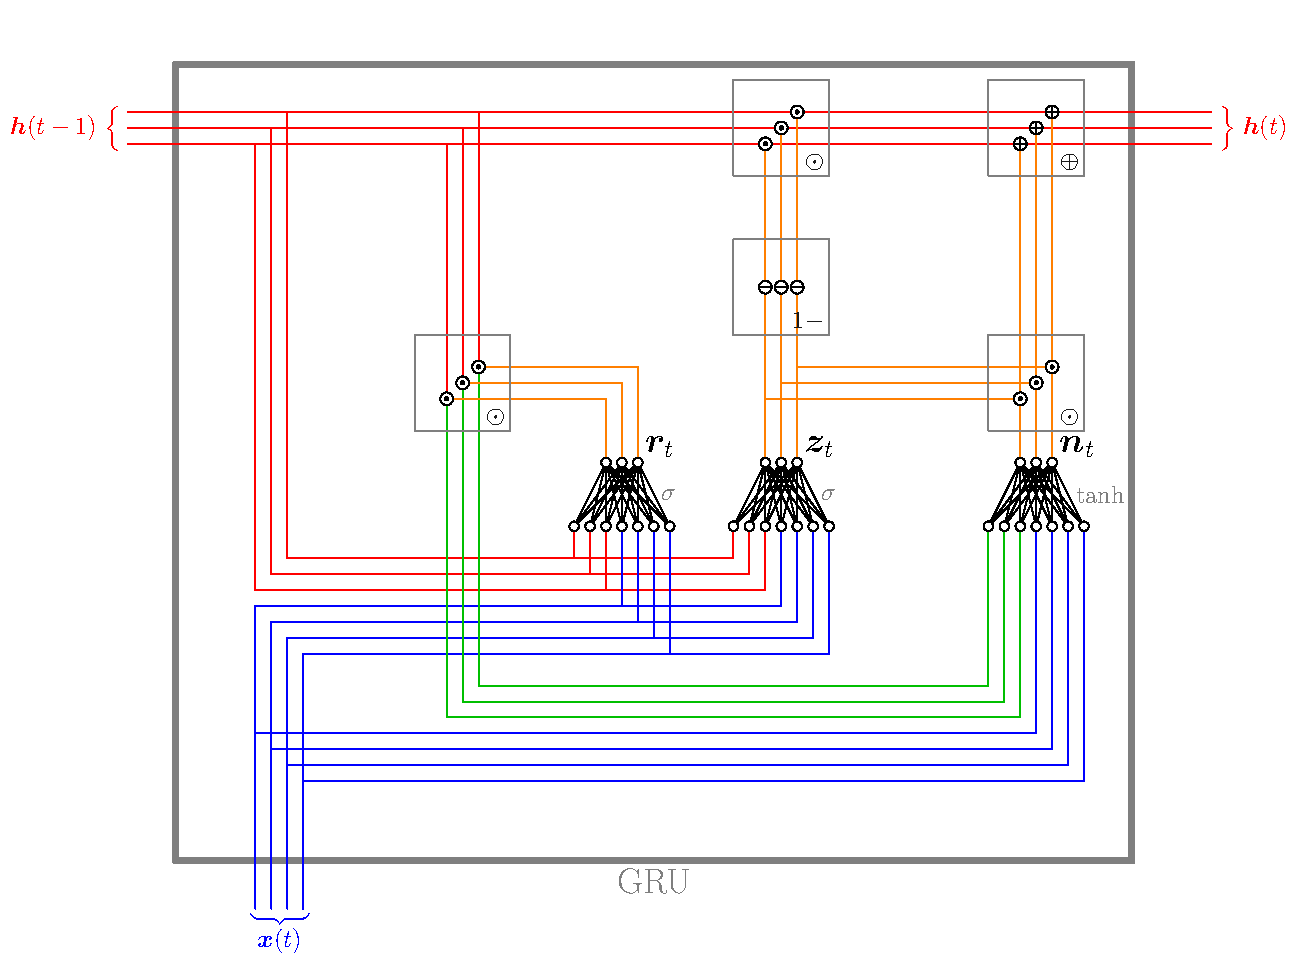
\includegraphics[width=8cm]{GRU.pdf}
\end{center}
\end{frame}
%-------------------------------------------------------------%

\begin{frame}[fragile]{pause}\frametitle{Gated Recurrent Unit (GRU)}
\begin{itemize}
\item $x_t$: input vector
\item $h_t$: output vector
\item $z_t$: update gate vector
\item $r_t$: reset gate vector
\item $W$, $U$, and $b$: parameter matrices and vector
\item $sigm$ or $\sigma_g$ is the sigmoid function
\item $tanh$ or $\sigma_h$ is the hyperbolic tangent
\end{itemize}
\end{frame}
%-------------------------------------------------------------%

\begin{frame}[fragile]{pause}\frametitle{Gated Recurrent Unit (GRU)}
Initially, for $t=0$, $h_0 = 0$
\begin{eqnarray}
z_t &=& \sigma_g (W_z x_t + U_z h_{t-1} + b_z)\nonumber\\\nonumber
r_t &=& \sigma_g (W_r x_t + U_r h_{t-1} + b_r)\\\nonumber
h_t &=& (1 - z_t) \odot h_{t-1} + z_t \odot \sigma_h (W_h x_t + U_h (r_t \odot h_{t-1}) + b_h) \nonumber
\end{eqnarray}
\end{frame}
%-------------------------------------------------------------%

\begin{frame}[fragile]{pause}\frametitle{GRU vs. LSTM?}
\begin{itemize}
\item GRUs have two gates (reset and update) whereas LSTM has three gates (input/output/forget)
\item GRU performance on par with LSTM but computationally more efficient (less complex).
\item In general, if you have a very large dataset then LSTMs will likely perform better. 
\item GRUs are a good choice for smaller datasets.
\end{itemize}
\end{frame}
%-------------------------------------------------------------%

\begin{frame}[fragile]{pause}\frametitle{Regularization in RNNs with LSTM units}
\begin{center}
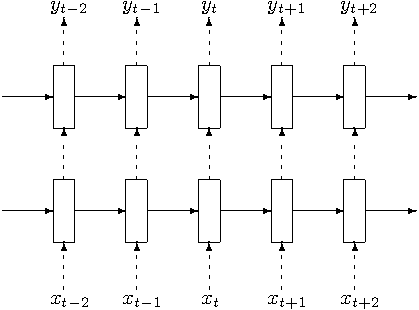
\includegraphics{reg_lstms.pdf}\footnote{\url{https://arxiv.org/pdf/1409.2329.pdf}}
\end{center}
\end{frame}
%-------------------------------------------------------------%

\begin{frame}[fragile]{pause}\frametitle{Regularization in RNNs with LSTM units}
\begin{center}
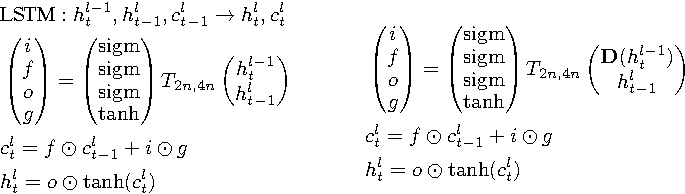
\includegraphics{reglstm_dropout.pdf}\footnote{\url{https://arxiv.org/pdf/1409.2329.pdf}}
\end{center}
\end{frame}
%-------------------------------------------------------------%

\end{document}